226. \begin{figure}[ht!]
\center{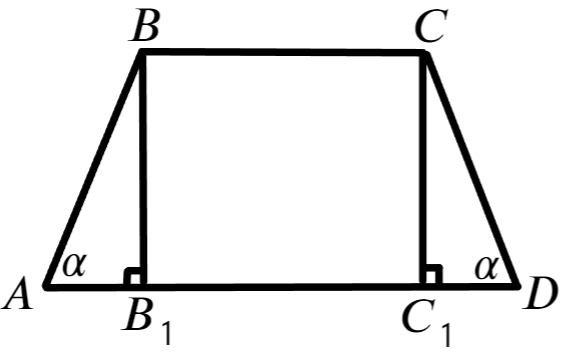
\includegraphics[scale=0.35]{g8-225.png}}
\end{figure}\\
Опустим высоты $BB_1$ и $CC_1.$ Так как трапеция равнобедренная, $AB_1=C_1D=\cfrac{b-a}{2}.$ Тогда боковые стороны трапеции равны $\cfrac{b-a}{2\cos(\alpha)},$
а высота равна $\cfrac{b-a}{2}\tg(\alpha).$ Таким образом, периметр трапеции равен $2\cdot\cfrac{b-a}{2\cos(\alpha)}+a+b=a+b+\cfrac{b-a}{\cos(\alpha)},$ высота равна $\cfrac{b-a}{2}\tg(\alpha),$ а площадь равна $\cfrac{b-a}{2}\tg(\alpha)\cdot\cfrac{a+b}{2}=\cfrac{(b^2-a^2)\tg(\alpha)}{4}.$\\
